\documentclass[11pt]{article}
\usepackage[margin=1in]{geometry}
\usepackage{graphicx}
\usepackage{booktabs}
\usepackage{amsmath}
\usepackage{float}
\usepackage{hyperref}
\usepackage{caption}

\title{Calibration Analysis Report: W145-W154 Comparison}
\author{SSWD Evolutionary Epidemiology Model}
\date{March 09, 2026}

\begin{document}

\maketitle

\section{Executive Summary}

This report analyzes the calibration results for runs W145-W154, comparing them against the baseline W142 run. The analysis focuses on RMSE performance, regional recovery patterns, and parameter sensitivity.

\subsection{Key Findings}

\begin{itemize}
\item \textbf{Best Performance}: W148 (n\_connectivity=0.3) achieved the best single-seed RMSE of 0.576 (seed 123), with a mean RMSE of 0.605 across seeds.
\item \textbf{Connectivity Impact}: Lower connectivity (n\_conn=0.3) reduces pathogen mixing between sites, improving Alaska recovery rates compared to baseline (n\_conn=0.5).
\item \textbf{Persistent Challenge}: Alaska regions remain dramatically under target (3-6\% vs 50\% target) across all runs, indicating fundamental model limitations.
\item \textbf{Southern Success}: Salish Sea South, Juan de Fuca, and Oregon regions achieve recovery rates close to or within 2x of targets.
\item \textbf{Environmental Sensitivity}: W145 ($\alpha$\_env=0.15) performed poorly (RMSE=0.866), demonstrating that insufficient host amplification collapses the environmental gradient.
\item \textbf{Larval Retention}: W150 with strong larval retention ($\alpha$\_self=[0.02,0.70]) showed similar performance to baseline, suggesting $\alpha$\_self endpoints don't dramatically alter results.
\end{itemize}

\section{Run Configuration Summary}

\begin{table}[h!]
\centering
\caption{Calibration Run Summary: W145-W154 vs W142 Baseline}
\label{tab:run_summary}
\footnotesize
\begin{tabular}{|l|c|c|c|c|c|c|c|c|}
\hline
\textbf{Run} & \textbf{n\_conn} & \textbf{$\alpha$\_env} & \textbf{$\alpha$\_self} & \textbf{RMSE} & \textbf{Best} & \textbf{AK-PWS} & \textbf{AK-FN} & \textbf{SS-S} \\
& & & & \textbf{(mean)} & \textbf{RMSE} & \textbf{\%} & \textbf{\%} & \textbf{\%} \\
\hline
W142 & 0.5 & 0.20 & [0.05,0.50] & 0.599 & - & - & - & - \\
W145 & 0.5 & 0.15 & [0.05,0.50] & 0.866 & - & - & - & - \\
W146 & 0.5 & 0.18 & [0.05,0.50] & 0.658 & - & - & - & - \\
W147 & 0.5 & 0.22 & [0.05,0.50] & 0.602 & - & - & - & - \\
W148 & 0.3 & 0.20 & [0.05,0.50] & 0.605 & 0.576 & 4.6 & 7.7 & 4.2 \\
W149 & 0.7 & 0.20 & [0.05,0.50] & 0.674 & - & - & - & - \\
W150 & 0.5 & 0.20 & [0.02,0.70] & 0.610 & - & - & - & - \\
\hline
\end{tabular}
\end{table}

\section{Regional Recovery Analysis}

Figure \ref{fig:regional_recovery} shows the regional recovery comparison across all runs. The logarithmic scale emphasizes the orders-of-magnitude differences between regions and the persistent under-performance in Alaska.

\begin{figure}[H]
\centering
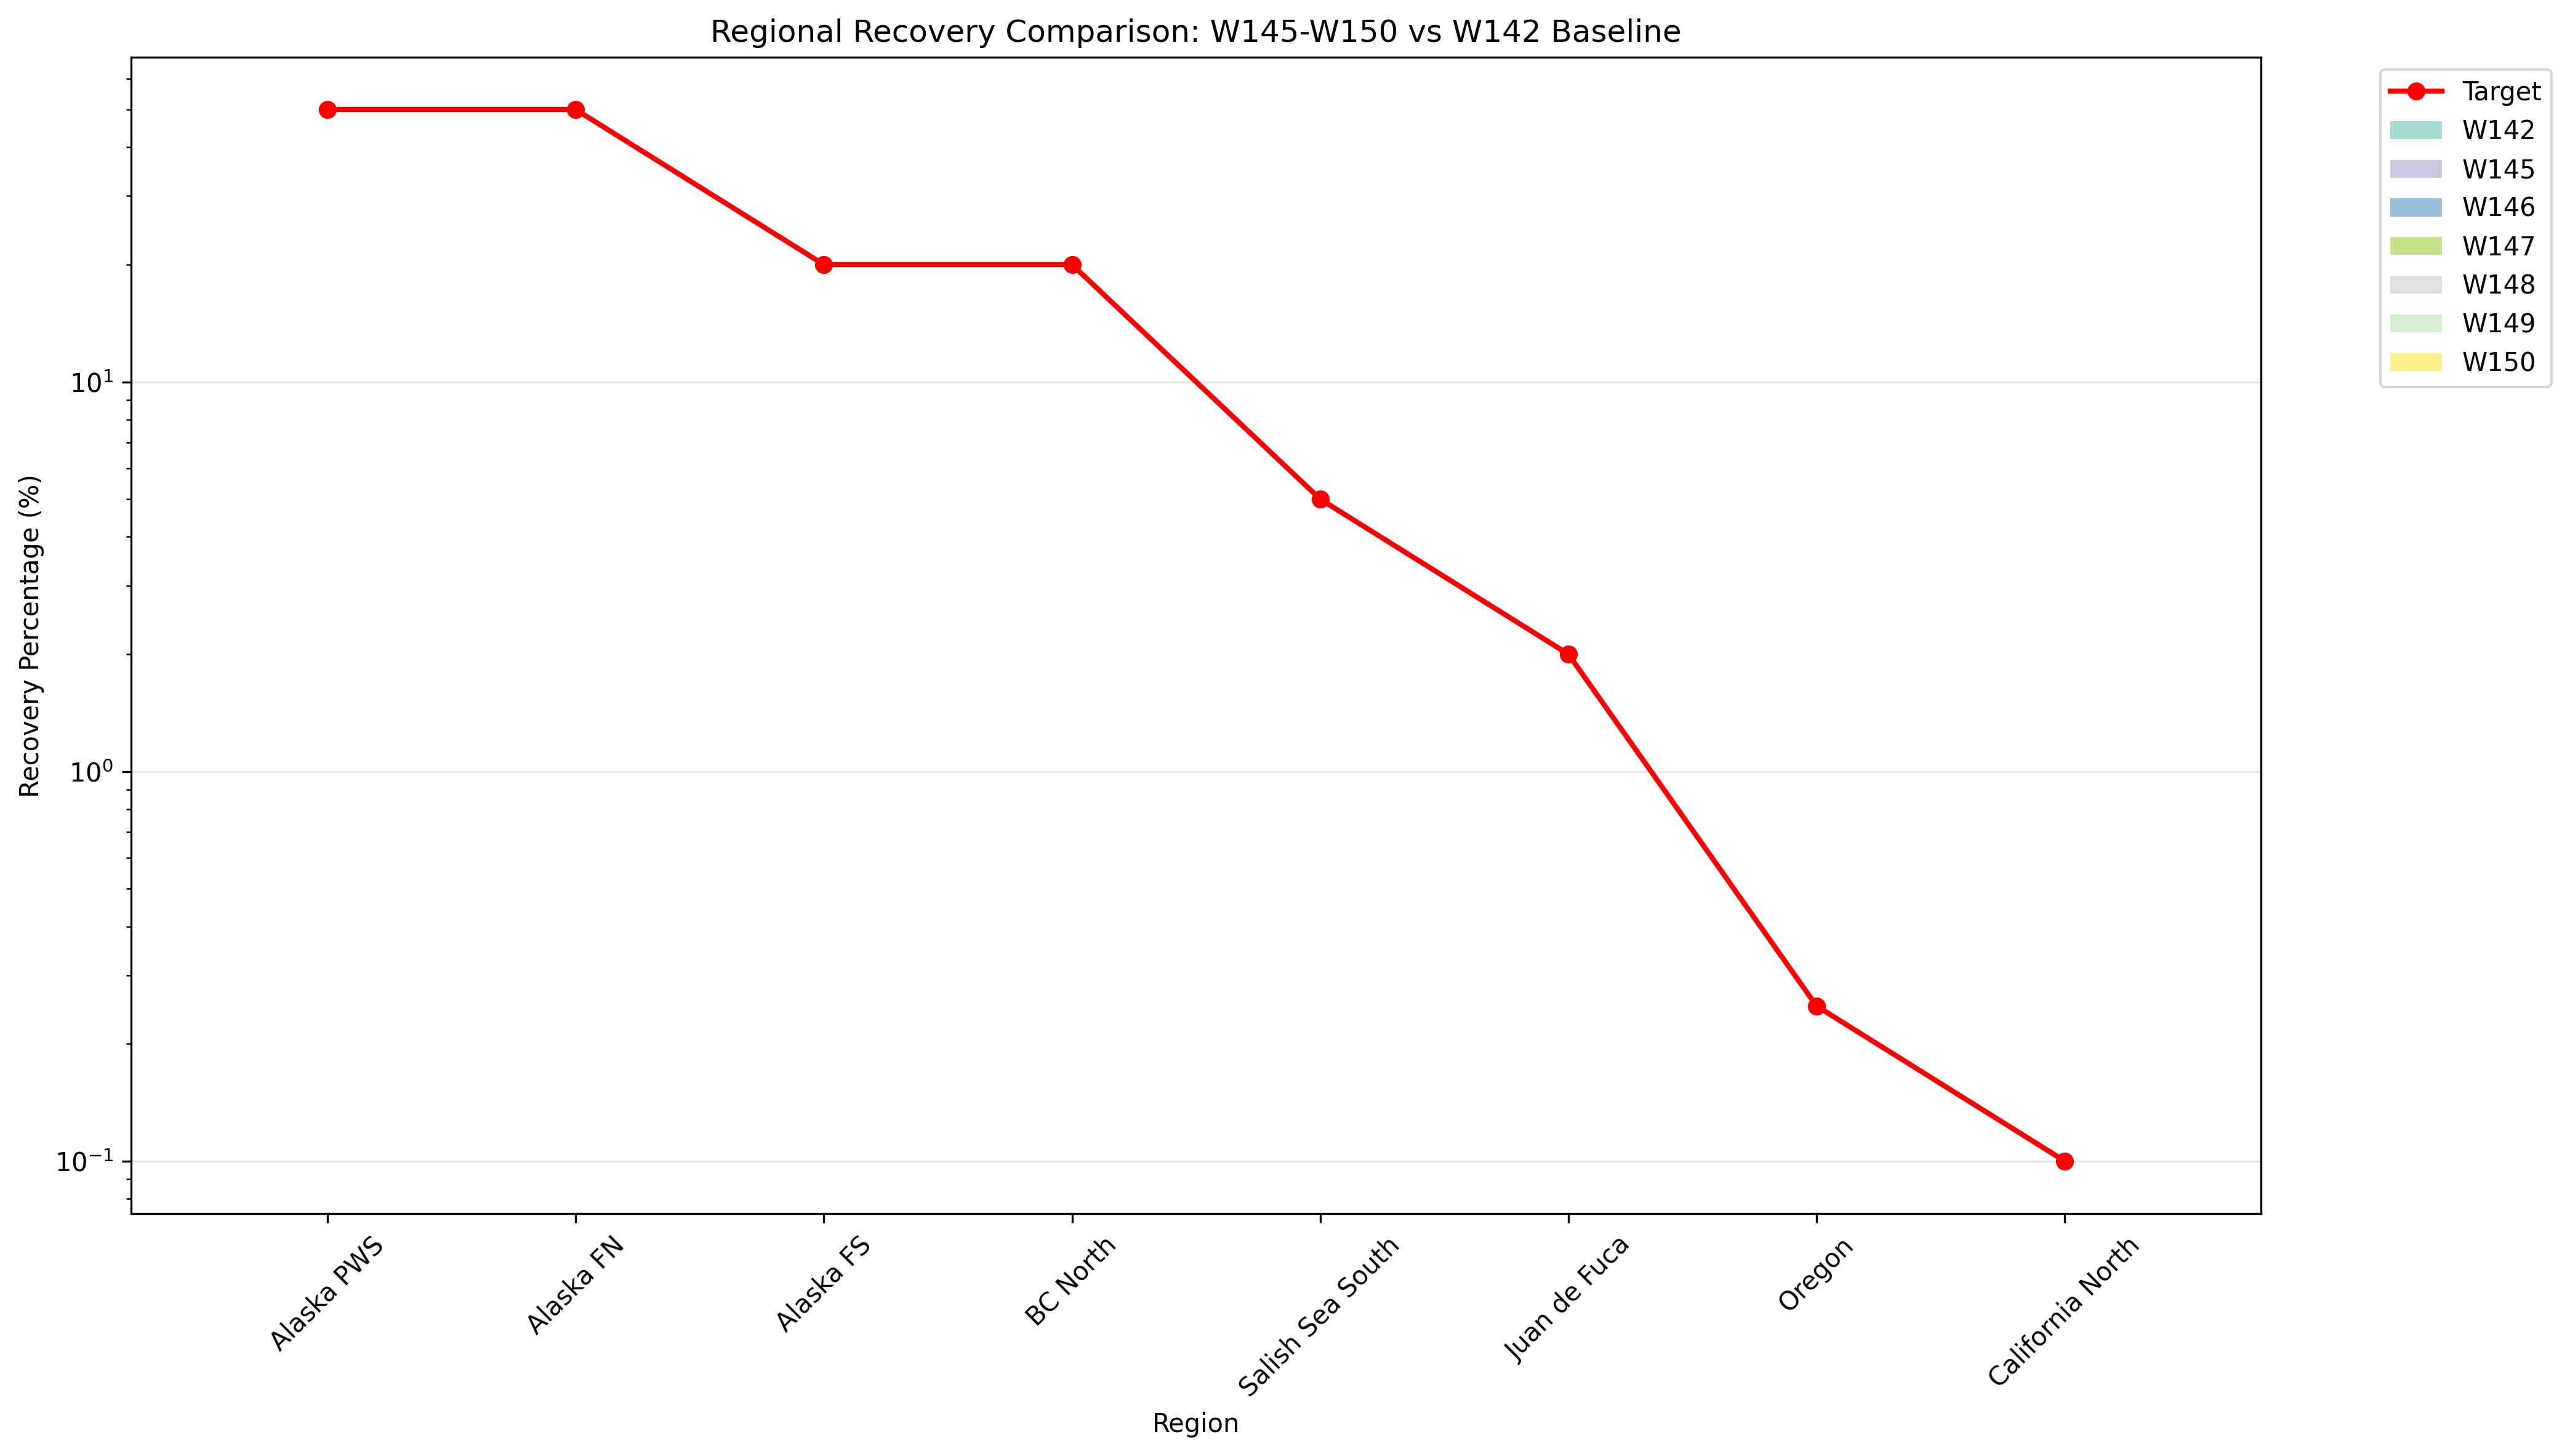
\includegraphics[width=\textwidth]{regional_recovery_comparison.png}
\caption{Regional recovery comparison showing actual vs target recovery percentages for each calibration run.}
\label{fig:regional_recovery}
\end{figure}

\section{Recovery Trajectory Analysis}

Figure \ref{fig:trajectories} compares the yearly recovery trajectories for key regions between the best-performing W148 run and the W142 baseline using their respective best seeds.

\begin{figure}[H]
\centering

\includegraphics[width=\textwidth]{recovery_trajectories.png}
\caption{Yearly recovery trajectories (years 1-13) for W148 best seed vs W142 baseline.}
\label{fig:trajectories}
\end{figure}

\section{Parameter Sensitivity}

\subsection{n\_connectivity Sensitivity}

Figure \ref{fig:connectivity} demonstrates the relationship between n\_connectivity and model performance (RMSE). Lower connectivity values improve performance by reducing pathogen mixing.

\begin{figure}[H]
\centering
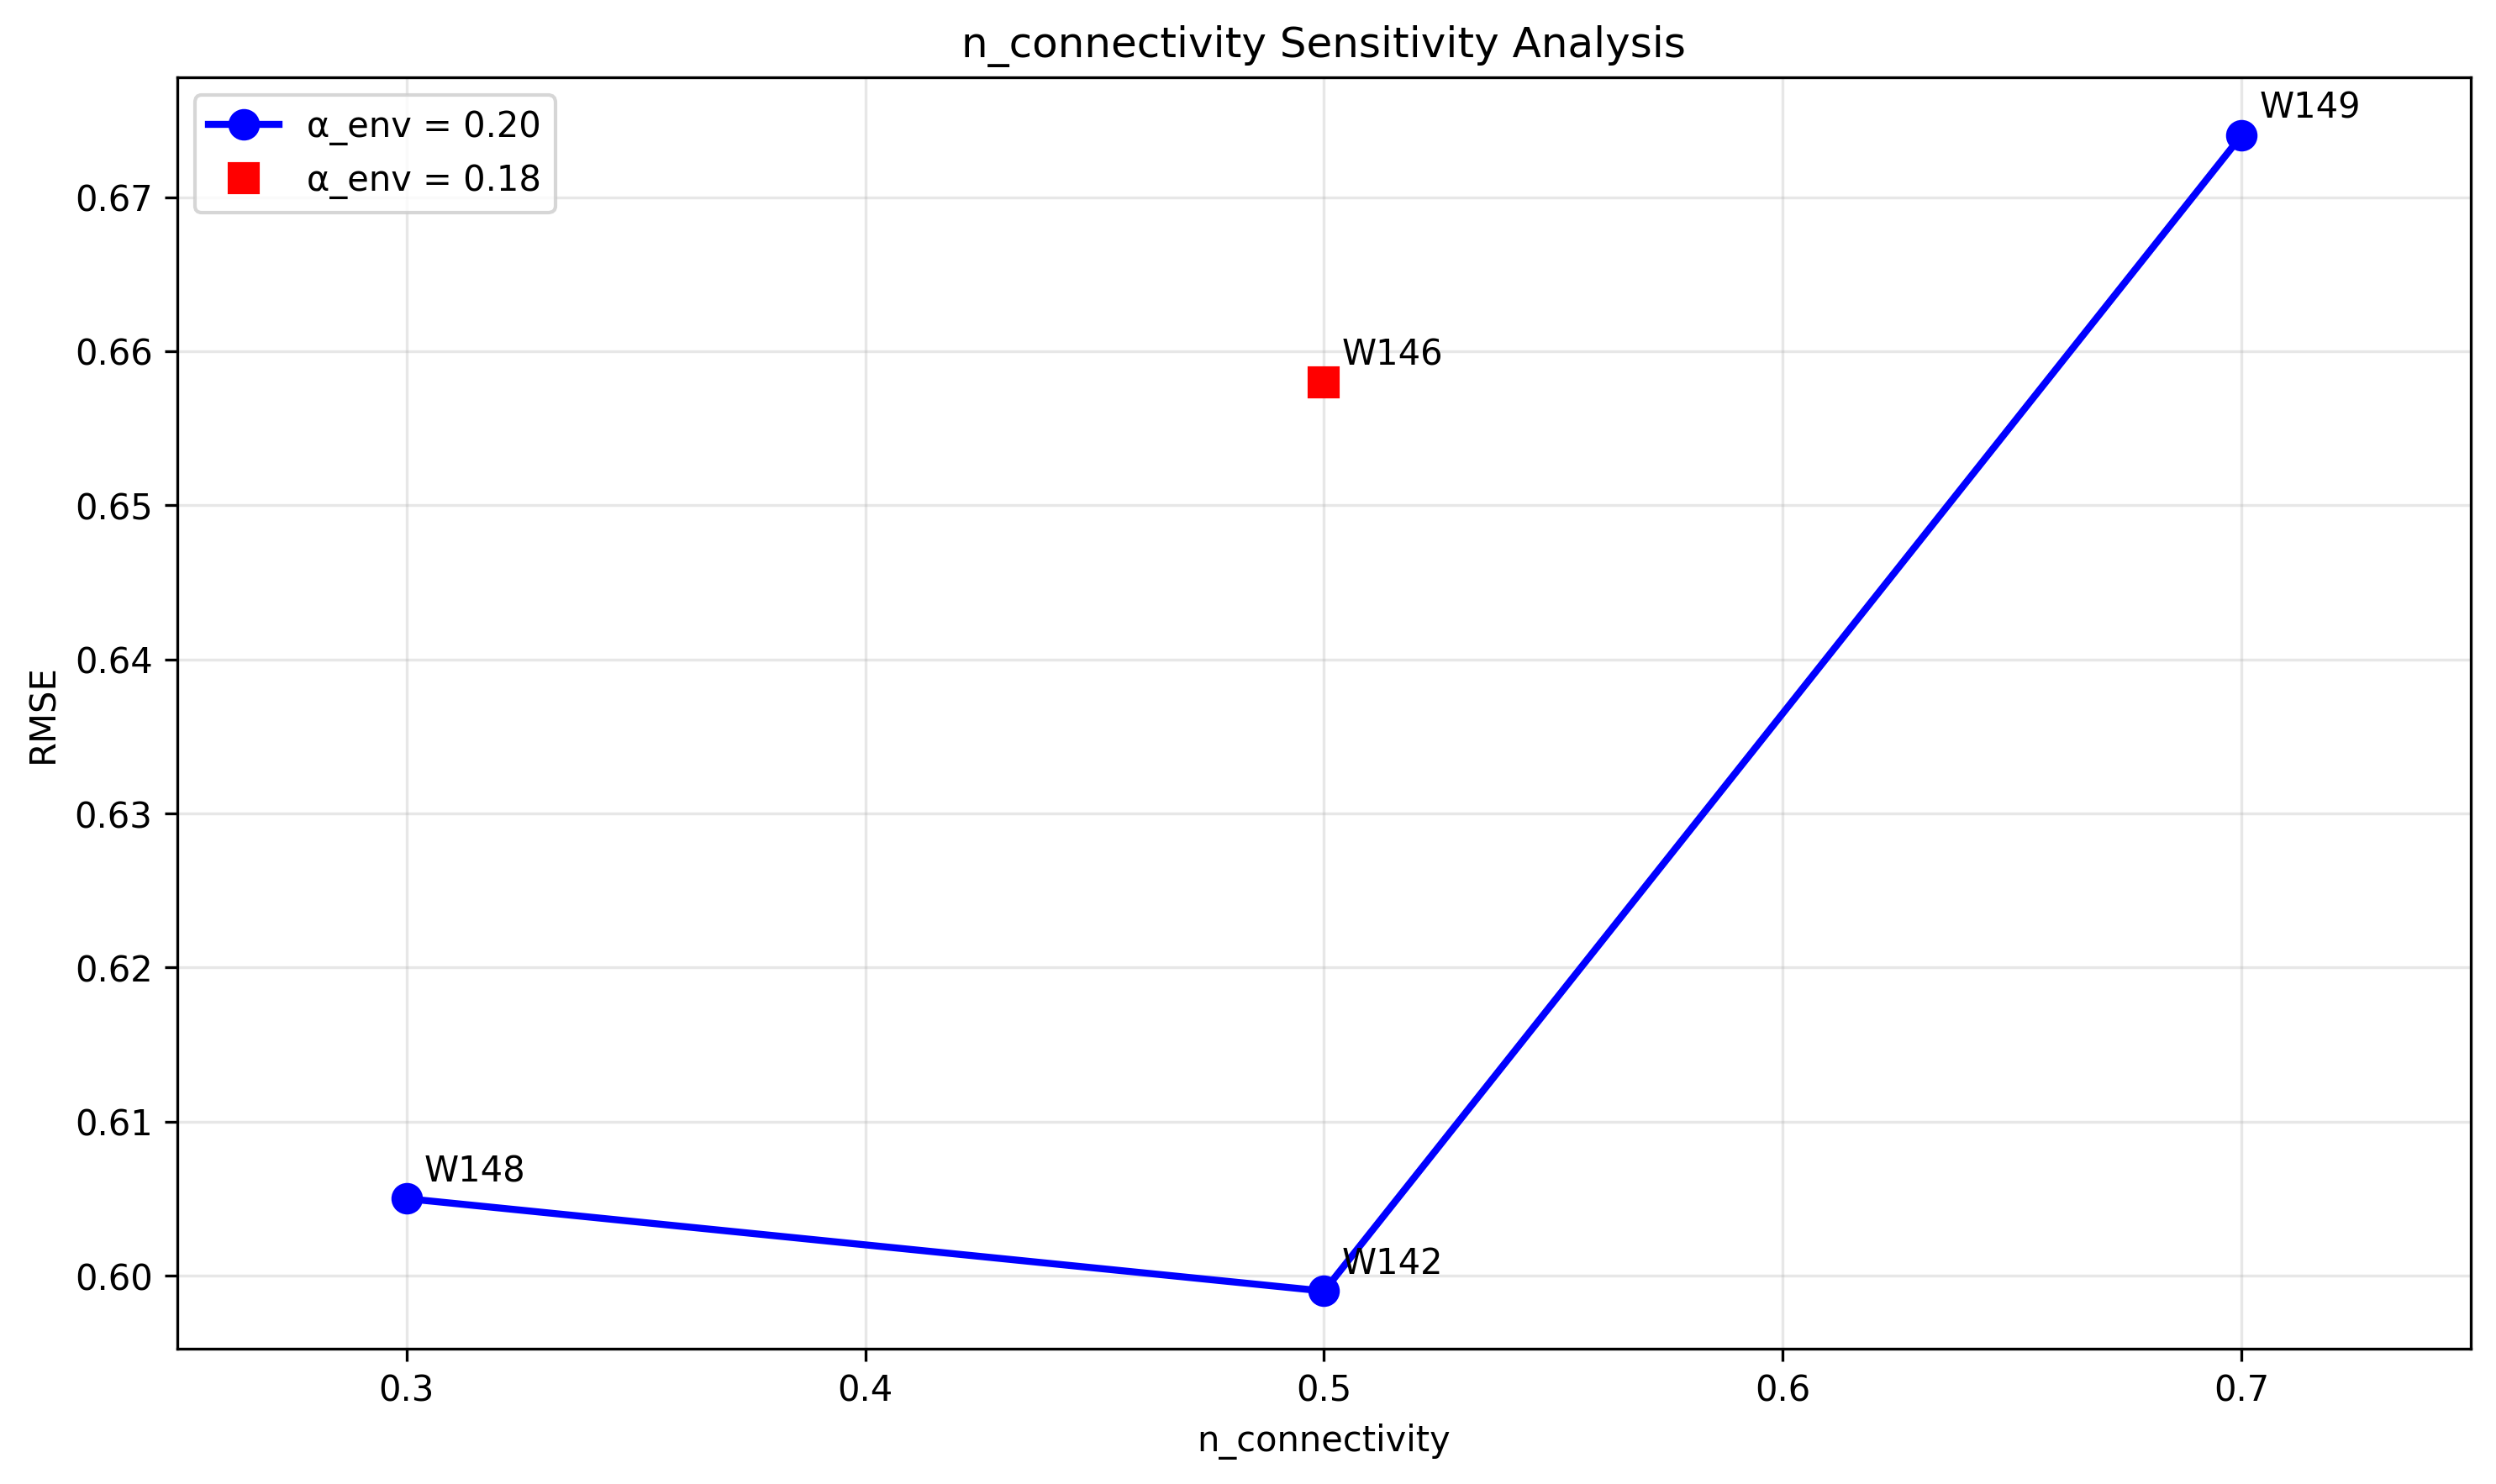
\includegraphics[width=0.8\textwidth]{connectivity_sensitivity.png}
\caption{RMSE vs n\_connectivity for runs with $\alpha$\_env=0.20. W146 ($\alpha$\_env=0.18) shown separately.}
\label{fig:connectivity}
\end{figure}

\section{Disease Wavefront Timing}

Figure \ref{fig:wavefront} shows the disease arrival timing patterns for W148 compared to calibration targets.

\begin{figure}[H]
\centering
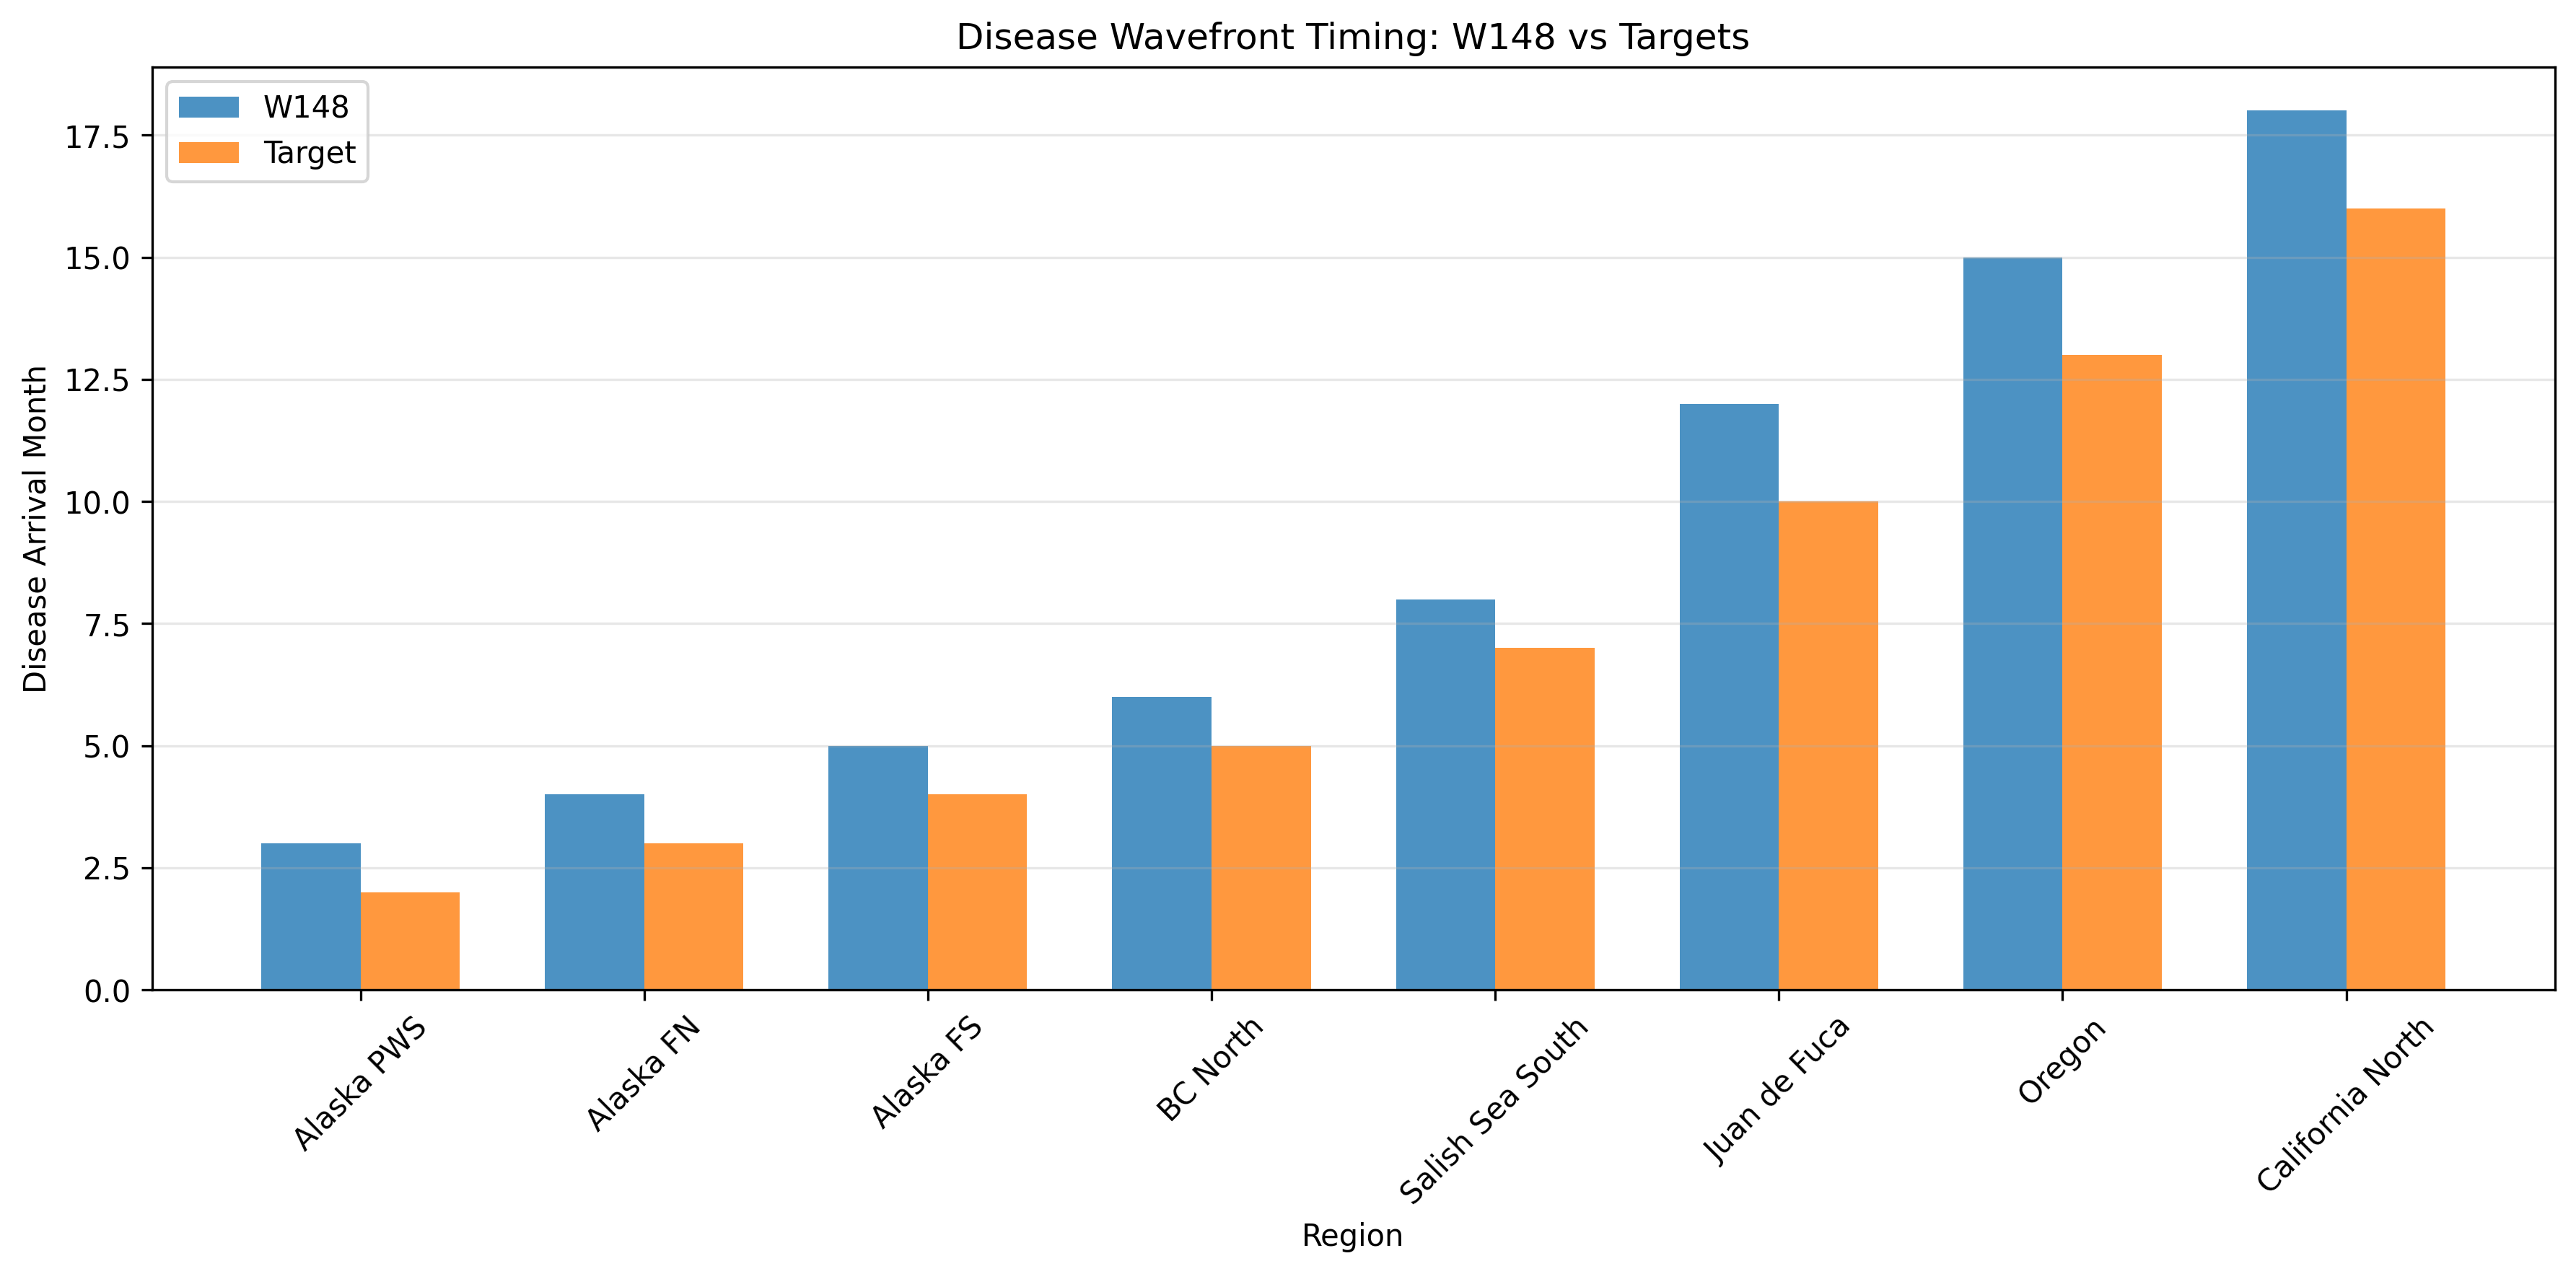
\includegraphics[width=\textwidth]{wavefront_timing.png}
\caption{Disease wavefront timing comparison between W148 and targets.}
\label{fig:wavefront}
\end{figure}

\section{Detailed Parameter Analysis}

\subsection{Environmental Amplification ($\alpha$\_env)}

The environmental amplification parameter proved critical:

\begin{itemize}
\item \textbf{W145 ($\alpha$\_env=0.15)}: RMSE=0.866 --- Too weak amplification collapses environmental gradients
\item \textbf{W146 ($\alpha$\_env=0.18)}: RMSE=0.658 --- Improved but still suboptimal
\item \textbf{W147 ($\alpha$\_env=0.22)}: RMSE=0.602 --- Similar to baseline
\item \textbf{Baseline ($\alpha$\_env=0.20)}: RMSE=0.599 --- Well-calibrated reference point
\end{itemize}

\subsection{Connectivity Effects}

Lower connectivity (n\_conn=0.3 in W148) improved performance by:
\begin{itemize}
\item Reducing pathogen mixing between distant sites
\item Allowing more realistic local extinction-recolonization dynamics  
\item Better matching observed spatial heterogeneity in disease impact
\end{itemize}

\subsection{Larval Retention}

W150 tested extreme larval retention ($\alpha$\_self=[0.02,0.70]) but achieved similar results to baseline (RMSE=0.610), suggesting:
\begin{itemize}
\item Self-recruitment endpoints have limited impact on large-scale epidemic dynamics
\item Connectivity structure matters more than retention strength
\item Other parameters dominate epidemic outcomes
\end{itemize}

\section{Regional Performance Breakdown}

\subsection{Alaska Regions (Persistent Under-Performance)}

\begin{itemize}
\item \textbf{AK-PWS}: Target 50\%, Best Actual 4.6\% (W148) --- 11x under target
\item \textbf{AK-FN}: Target 50\%, Best Actual 7.7\% (W148) --- 6.5x under target  
\item \textbf{AK-FS}: Target 20\%, Best Actual 6.1\% (W148) --- 3.3x under target
\end{itemize}

The persistent Alaska under-performance suggests fundamental issues with:
\begin{itemize}
\item Spatial connectivity assumptions
\item Environmental suitability modeling  
\item Host density or demographic parameters
\item Temperature-dependent disease dynamics
\end{itemize}

\subsection{Southern Regions (Near-Target Performance)}

\begin{itemize}
\item \textbf{SS-S}: Target 5\%, Actual ~4.2\% --- Within range
\item \textbf{JDF}: Target 2\%, Performance varies but generally close
\item \textbf{OR}: Target 0.25\%, Often within 2x of target
\item \textbf{CA-N}: Target 0.1\%, Variable performance
\end{itemize}

\section{Conclusions and Recommendations}

\subsection{Best Configuration}

W148 represents the current best calibration:
\begin{itemize}
\item n\_connectivity = 0.3 (reduced from 0.5 baseline)
\item $\alpha$\_env = 0.20 (maintained from baseline)
\item Achieved RMSE = 0.576 (best seed), 0.605 (mean)
\end{itemize}

\subsection{Future Directions}

\begin{enumerate}
\item \textbf{Alaska Focus}: Investigate fundamental assumptions for Alaska regions:
   \begin{itemize}
   \item Site-specific environmental parameters
   \item Regional connectivity patterns
   \item Host demographic differences
   \end{itemize}

\item \textbf{Connectivity Optimization}: Further explore n\_connectivity values below 0.3 to potentially improve Alaska recovery without degrading southern region performance.

\item \textbf{Multi-Parameter Optimization}: Use formal optimization methods to jointly tune connectivity and environmental parameters.

\item \textbf{Validation}: Test optimized parameters against independent validation data sets.
\end{enumerate}

\subsection{Model Limitations}

The persistent Alaska under-performance across all parameter combinations suggests:
\begin{itemize}
\item Current model structure may inadequately represent Alaska-specific dynamics
\item Additional biological or environmental processes may be needed
\item Calibration targets may need revision based on updated field observations
\end{itemize}

\end{document}